\pagebreak
\restoregeometry 
\section{Modelos de reducción de dimensiones.}

\subsection{Análisis de componentes principales (PCA)}

Al hacer el análisis de componentes principales a los datos se obtuvieron las siguientes cargas en las primeras dos componentes. La varianza acumulada en las primeras dos componentes es del $83.59 \%$ y se considera suficiente para el análisis.
Como se puede observar la primera componente está asociada con la ceniza, el sodio y la proteína, mientras que la segunda se asocia con la humedad, los carbohidratos y las calorías.
Las componentes principales se obtuvieron usando la función \textsf{prcomp} de R con los datos normalizados, la normalización no afectó drásticamente la representación gráfica, sin embargo, permitió observar de forma más clara las relaciones entre las variables ya mencionadas.


\begin{table}[ht]
\centering
\begin{tabular}{rrr}
  \hline
 & PC1 & PC2 \\ 
  \hline
Humedad & 0.21 & 0.58 \\ 
  Proteina & -0.47 & -0.03 \\ 
  Grasa & -0.19 & 0.41 \\ 
  Ceniza & -0.51 & 0.15 \\ 
  Sodio & -0.47 & -0.02 \\ 
  Carbohidratos & 0.32 & -0.49 \\ 
  Calorias & -0.34 & -0.48 \\ 
  Varianza acumulada & 48.64 \% &  83.59 \% \\ 
\end{tabular}
	\label{tabla:pesos_PCA}
	\caption{Pesos asociados a las primeras dos componentes principales.}
\end{table}


\begin{figure}[h]
\centering
	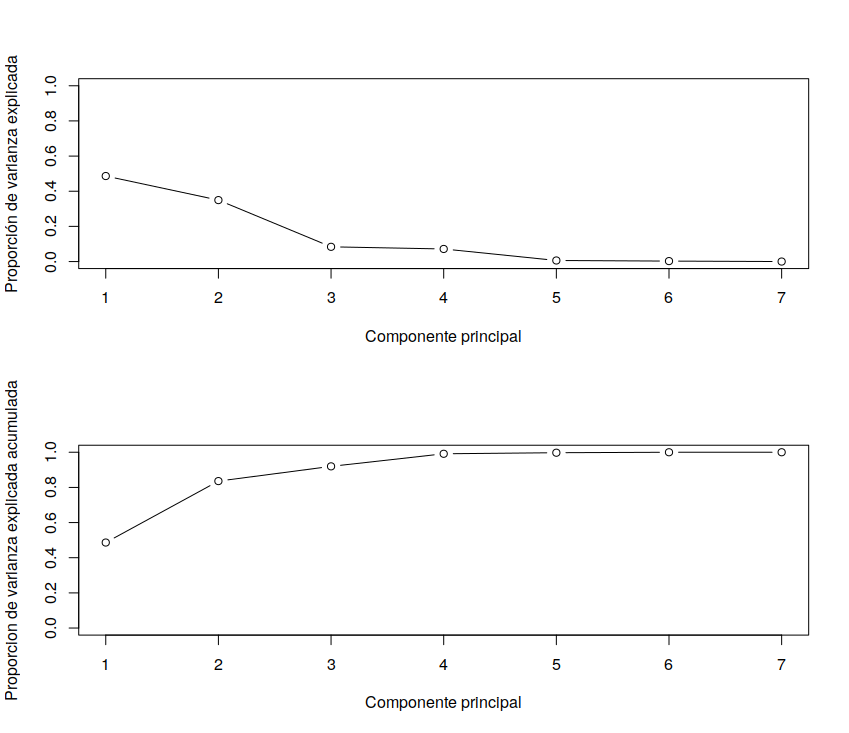
\includegraphics[scale=.5]{images/varPCA.png} 
	\label{i_var_PCA}
	\caption{Varianza explicada por las componentes principales}
\end{figure}

\subsubsection{Representación gráfica (biplot)}

La figura  \ref{i_biplot_PCA} muestra la representación en las primeras dos componentes principales de los datos, en ella se aprecia una clara separación entre algunos grupos de pizzas, específicamente, la marca A se distingue por tener altos niveles de sodio y proteina, las marcas B, C y D se caracterizan por un alto nivel de ceniza, E y F por tener altos valores de humedad, finalmente el resto de marcas (G, H, I, J, K y L) se distinguen por su alto contenido en carbohidratos. 
También el biplot muestra la alta colinealidad existente entre las variables sodio y proteina, y sugiere un contraste entre la variables grasa y carbohidratos.


\begin{figure}[h]
\centering
	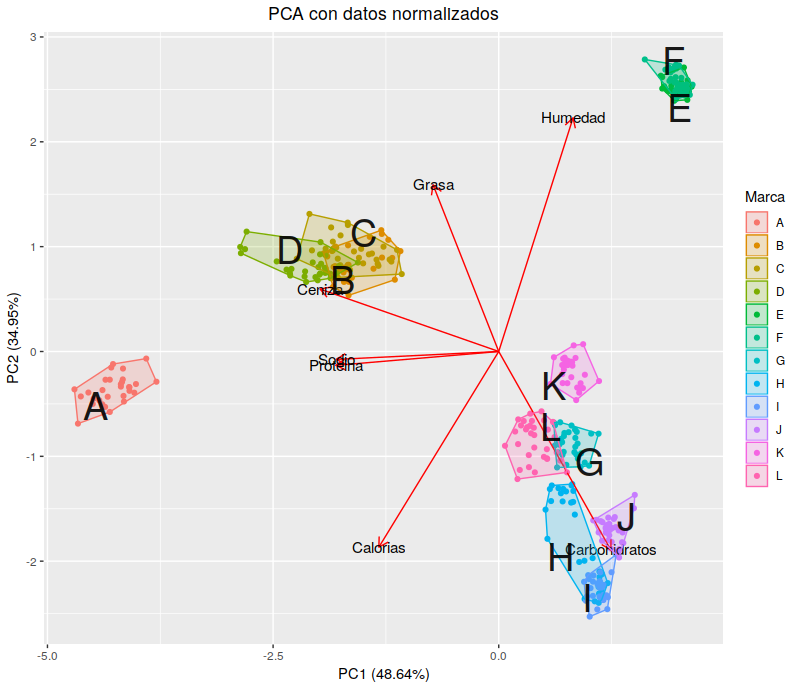
\includegraphics[scale=.75]{images/biplotPCA.png} 
	\label{i_biplot_PCA}
	\caption{Biplot PCA}
\end{figure}


\subsection{Análisis de factores}

Se realizó el análisis de factores usando dos factores, esto debido a la baja dimensión del problema.


\begin{table}[ht]
\centering
\begin{tabular}{rrrrr}
  \hline
 & Factor1 & Factor2 & Varianza específica & Comunalidades \\ 
  \hline
Humedad & 0.06 & -1.00 & 0.01 & 1.00 \\ 
  Proteina & 0.76 & 0.44 & 0.23 & 0.77 \\ 
  Grasa & 0.47 & -0.30 & 0.69 & 0.31 \\ 
  Ceniza & 0.94 & 0.19 & 0.08 & 0.92 \\ 
  Sodio & 0.73 & 0.39 & 0.32 & 0.68 \\ 
  Carbohidratos & -0.90 & 0.44 & 0.01 & 1.00 \\ 
  Calorias & 0.23 & 0.97 & 0.01 & 0.99 \\     
  Proporción de Varianza  & 44 \% &  36.9 \% \\
  Varianza acumulada & 44 \% &  80.9 \% \\ 
   \hline
\end{tabular}
\end{table}